% --------------------------------------
% Document Class
% --------------------------------------
\documentclass[a4paper,11pt]{article}
% --------------------------------------



% --------------------------------------
% Use Package
% --------------------------------------


\usepackage[francais]{babel}
%\usepackage{ucs}
\usepackage[utf8]{inputenc}
\usepackage[T1]{fontenc}

\usepackage{makeidx}
\usepackage{color}
\usepackage{graphicx}
\usepackage{float}
\usepackage[hidelinks]{hyperref} 
\usepackage{geometry}
%\usepackage{lastpage}
%\usepackage{marginnote}
\usepackage{fancyhdr}
%\usepackage{titlesec}
%\usepackage{framed}
\usepackage{amsmath}
\usepackage{empheq}
\usepackage{array}
\usepackage{multicol}
%\usepackage{adjustbox}

% insert code
\usepackage{listings}

% define our color
\usepackage{xcolor}

% code color
\definecolor{ligthyellow}{RGB}{250,247,220}
\definecolor{darkblue}{RGB}{5,10,85}
\definecolor{ligthblue}{RGB}{1,147,128}
\definecolor{darkgreen}{RGB}{8,120,51}
\definecolor{darkred}{RGB}{160,0,0}

% other color
\definecolor{ivi}{RGB}{141,107,185}


\lstset{
    language=Scilab,
    captionpos=b,
    extendedchars=true,
    frame=lines,
    numbers=left,
    numberstyle=\tiny,
    numbersep=5pt,
    keepspaces=true,
    breaklines=true,
    showspaces=false,
    showstringspaces=false,
    breakatwhitespace=false,
    stepnumber=1,
    showtabs=false,
    tabsize=3,
    basicstyle=\small\ttfamily,
    backgroundcolor=\color{ligthyellow},
    keywordstyle=\color{ligthblue},
    morekeywords={include, printf, uchar},
    identifierstyle=\color{darkblue},
    commentstyle=\color{darkgreen},
    stringstyle=\color{darkred},
}


% --------------------------------------



% --------------------------------------
% Page setting
% --------------------------------------
%\pagestyle{empty}
\setlength{\headheight}{15pt}

\setcounter{secnumdepth}{3}
\setcounter{tocdepth}{2}

\makeatletter
\@addtoreset{chapter}{part}
\makeatother 

\hypersetup{         % parametrage des hyperliens
  colorlinks=true,      % colorise les liens
  breaklinks=true,      % permet les retours à la ligne pour les liens trop longs
  urlcolor= blue,       % couleur des hyperliens
  linkcolor= black,     % couleur des liens internes aux documents (index, figures, tableaux, equations,...)
  citecolor= green      % couleur des liens vers les references bibliographiques
}

% --------------------------------------

% --------------------------------------
% Information
% --------------------------------------
\title{Compte-rendu TP3 TI : Images discrètes}
\author{Elliot VANEGUE et Gaëtan DEFLANDRE}
% --------------------------------------

\definecolor{myColor}{rgb}{0.5, 0.1, 0.75}

% --------------------------------------
% Begin content
% --------------------------------------
\begin{document}

% Set language to english
  \selectlanguage{francais}

  % Start the page counting
  \pagenumbering{arabic}

  \maketitle
  
  \mbox{}
  \newpage
  \clearpage
  
  \section*{Introduction}
  
  \section{Composantes d'une image couleur}
  Nous allons d'abord voir comment manipulé les composantes d'une image couleur à partir de l'image de calibrage
  de couleur fournit dans le TP. On peut voir que la taille de la variable contenant l'image est de 1 440 000,
  qui correspond à $<largeur> * <hauteur> * <nombre de canaux>$.\\
  
  Pour récupérer la composante d'une couleur en image de gris, il suffit de récupérer le vecteur d'une des composantes
  et de l'afficher seul. Nous avons ainsi une matrice avec les valeurs de rouge et vu que nous ne gardons qu'une matrice,
  l'image se transforme en dégradé de gris.\\
  
  \begin{figure}[H]
    \center
    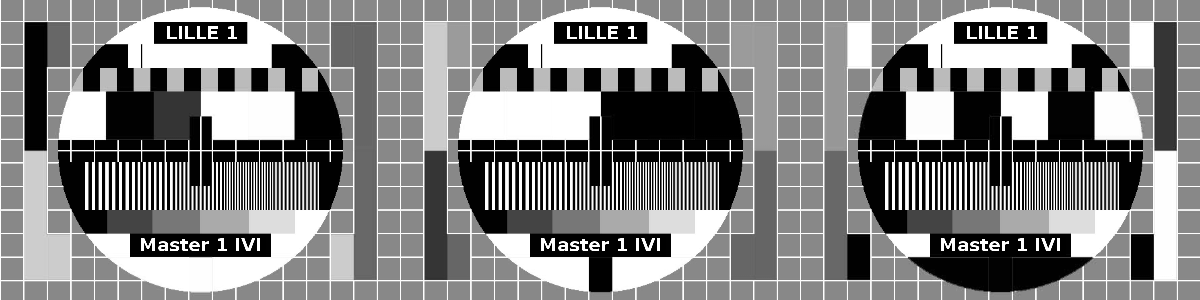
\includegraphics[width=10cm]{../mire_gris.png}
    \caption{Image en niveau de gris}
  \end{figure}
  
  La récupération d'une image dans un dégradé d'une seul couleur, il faut annuler les deux autres canaux en les multipliant par
  zéro.
  
  \begin{figure}[H]
    \center
    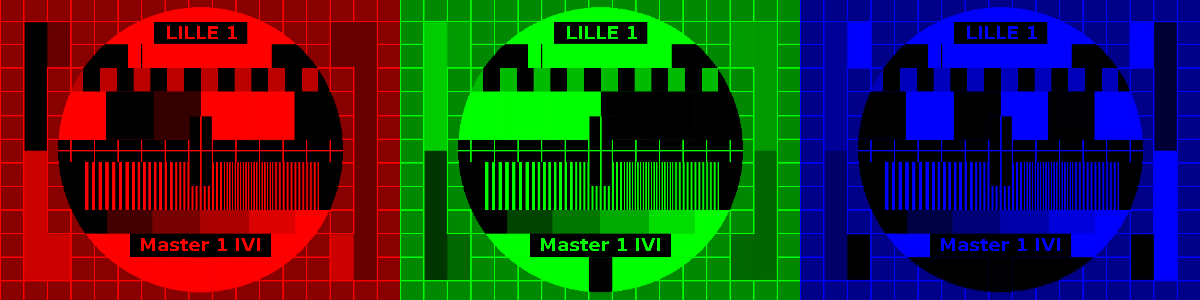
\includegraphics[width=10cm]{../mire_couleur.png}
    \caption{Image avec suppression de deux composantes de couleur}
  \end{figure}
  
  \section{Sur et sous-échantillonnage}
  Nous allons, avant de définir les notions de sur et sous-échantillonage, calculer les dimensions du support
  initial de l'image en prenant comme résolution d'acquisition 72 pixel/pouce. Ce calcul correspond à :
  <nb pixels sur x> / 72 et <nb pixels sur y> /72. Ce qui nous donne un support de 11x8 pouces.
  
  %800/72 = 11
  %600/72 = 8
  \subsection{Sous-échantillonage}
  Pour effectuer un sous-échantillonage, il faut supprimer un pixel tout les N pixels dans le vecteur de chaque canaux.
  Pour cela on récupère un vecteur avec l'ensemble des pixels de l'image, on en supprime le nombre nécessaire
  et on reforme la matrice de l'image.\\

  \begin{lstlisting}[caption=Fonction permettant le sous-échantillonnement d'une image]
    function [newImg] = sousEchant(img,n)
        s = size(img);
        newLenX = s(1)/n;
        newLenY = s(2)/n;
        newImg = zeros(newLenX,newLenY);
        for raw=1:newLenY
            for col=1:newLenX
                for c=1:s(3)
                    newImg(col,raw,c) = img(col*n,raw*n,c);
                end;
            end;
        end;
    endfunction;
  \end{lstlisting}
  
  \subsection{Sur-échantillonage}
  L'algorithme de sur-échantillonner d'une image doit prendre un groupe de pixels afin de faire la moyenne de leur valeur
  pour un canal. Ensuite, il suffit de créer un pixel au centre de ce groupe avec comme valeur la moyenne précédement calculer.
  Pour déterminer les groupes de pixel, il faut diviser le nombre de pixel sur une ligne par N et faire pareil sur une colonne.
  Ainsi les pixels ajouté auront une distance régulière avec une valeur moyenne.\\
  
  \begin{lstlisting}[caption=Fonction permettant le sur-échantillonnement d'une image]
    function [newImg] = surEchant(img,n)
        s = size(img);
        newLenX = s(1)/n;
        newLenY = s(2)/n;
        newImg = zeros(newLenX,newLenY);
        for raw=1:newLenY
            for col=1:newLenX
                for c=1:s(3)
                    if modulo(n,2) == 0 then
                        tabMoyenne = [img(col+1,raw,c) img(col-1,raw,c) img(col,raw+1,c) img(col,raw-1,c)]
                        newImg(col,raw,c) = mean(tabMoyenne);    
                    else
                        newImg(col,raw,c) = img(col-((n-1)*col),raw-((n-1)*raw),c);
                    end;
                end;
            end;
        end;
    endfunction;
  \end{lstlisting}
  
  \subsection{Cumulation d'échantillonage}
  %TODO faire les tests
  
  \section{Quantification}
  La quantification permet de déterminer le nombre de bit qui vont codé une composante. Cette variation
  va influencer le nombre de couleur qui seront présente dans l'image car si le nombre de bit qui code
  une composante diminu alors le nombre de valeur disponible pour cette composante diminu également.
  
  %TODO verif algo et test sur image
  \section{Repliement de spectre}
  %question 1 pixel/m -> resPeriode / 150
  
  \section*{Conclusion}
 
    
\end{document}  